\begin{tcolorbox}
In diesem Kapitel werden erste Skizzen (Mockups) der Benutzeroberflächen dargestellt.
Diese sollen in erster Linie dazu dienen, dem Kunden einen Überblick über die zu erstellenden UIs zu geben und ggf. Änderungen frühzeitig durchführen zu können.
Dafür eignen sich spezielle Tools, wie z.B. Balsamiq Mockups\footnote{\url{https://balsamiq.com/products/mockups}}.
\end{tcolorbox}

\begin{figure}[h]
\begin{tabularx}{\textwidth}{X | X}
	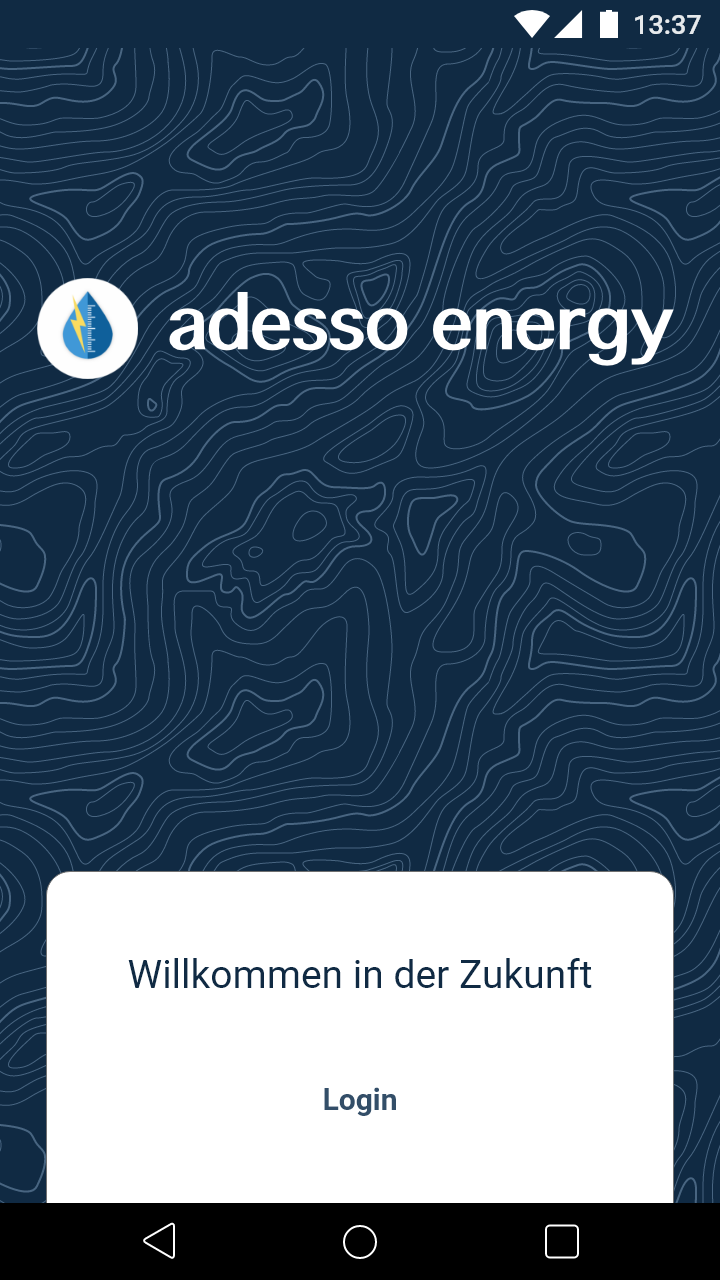
\includegraphics[scale = 0.22]{img/AndroidMockup/splash} & Ganz viel Text. Ganz viel Text.Ganz viel Text.Ganz viel Text.Ganz viel Text.Ganz viel Text.Ganz viel Text.Ganz viel Text. \\ \hline \\
	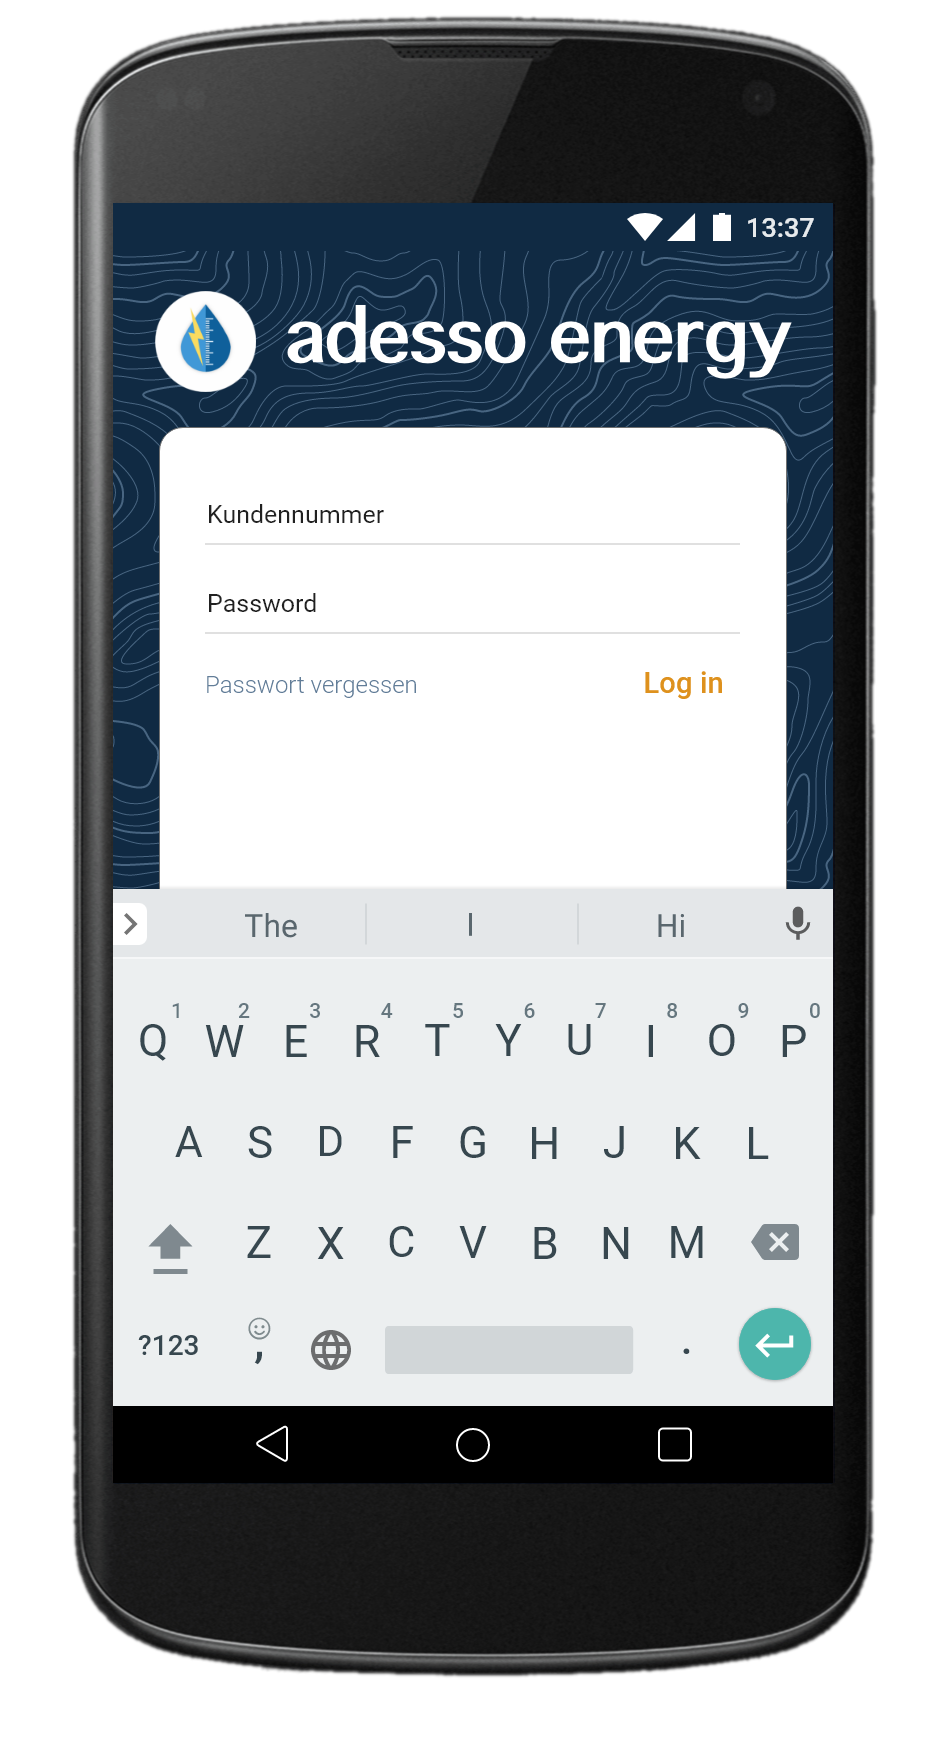
\includegraphics[scale = 0.22]{img/AndroidMockup/login} & Dies ist der LoginBildschirm \\ 
\end{tabularx}
\end{figure}


\begin{figure}[h]
\begin{tabularx}{\textwidth}{X | X}
	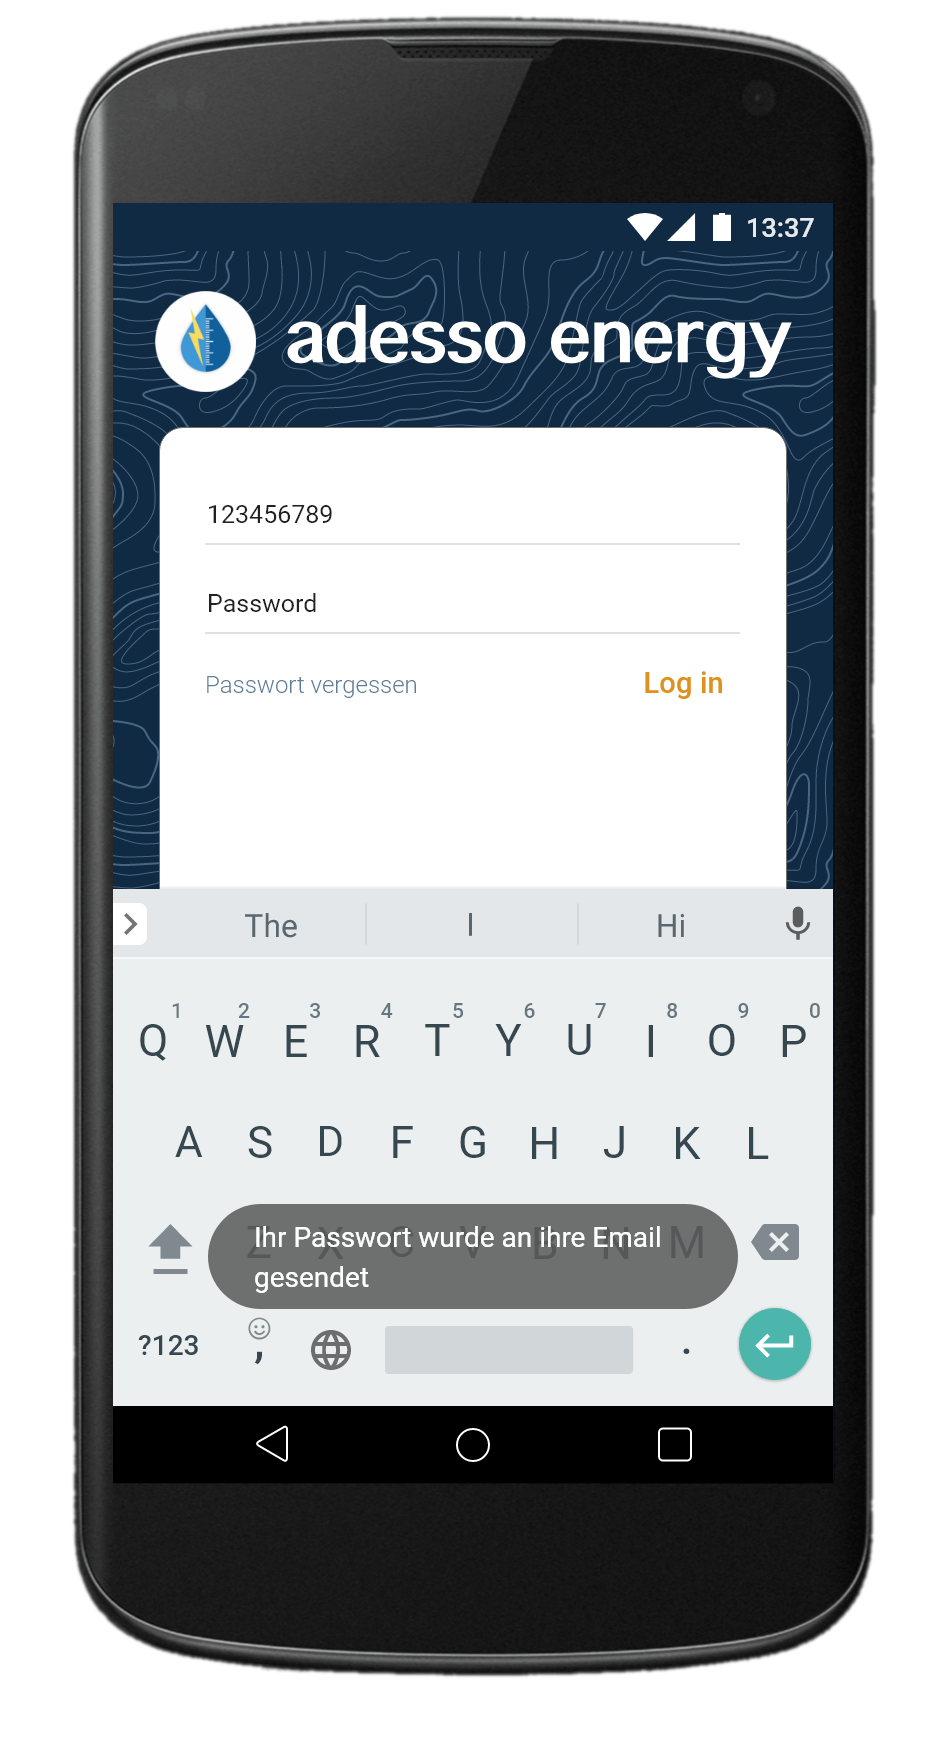
\includegraphics[scale = 0.22]{img/AndroidMockup/forgotPassword} & Ganz viel Text. Ganz viel Text.Ganz viel Text.Ganz viel Text.Ganz viel Text.Ganz viel Text.Ganz viel Text.Ganz viel Text. \\ \hline \\
	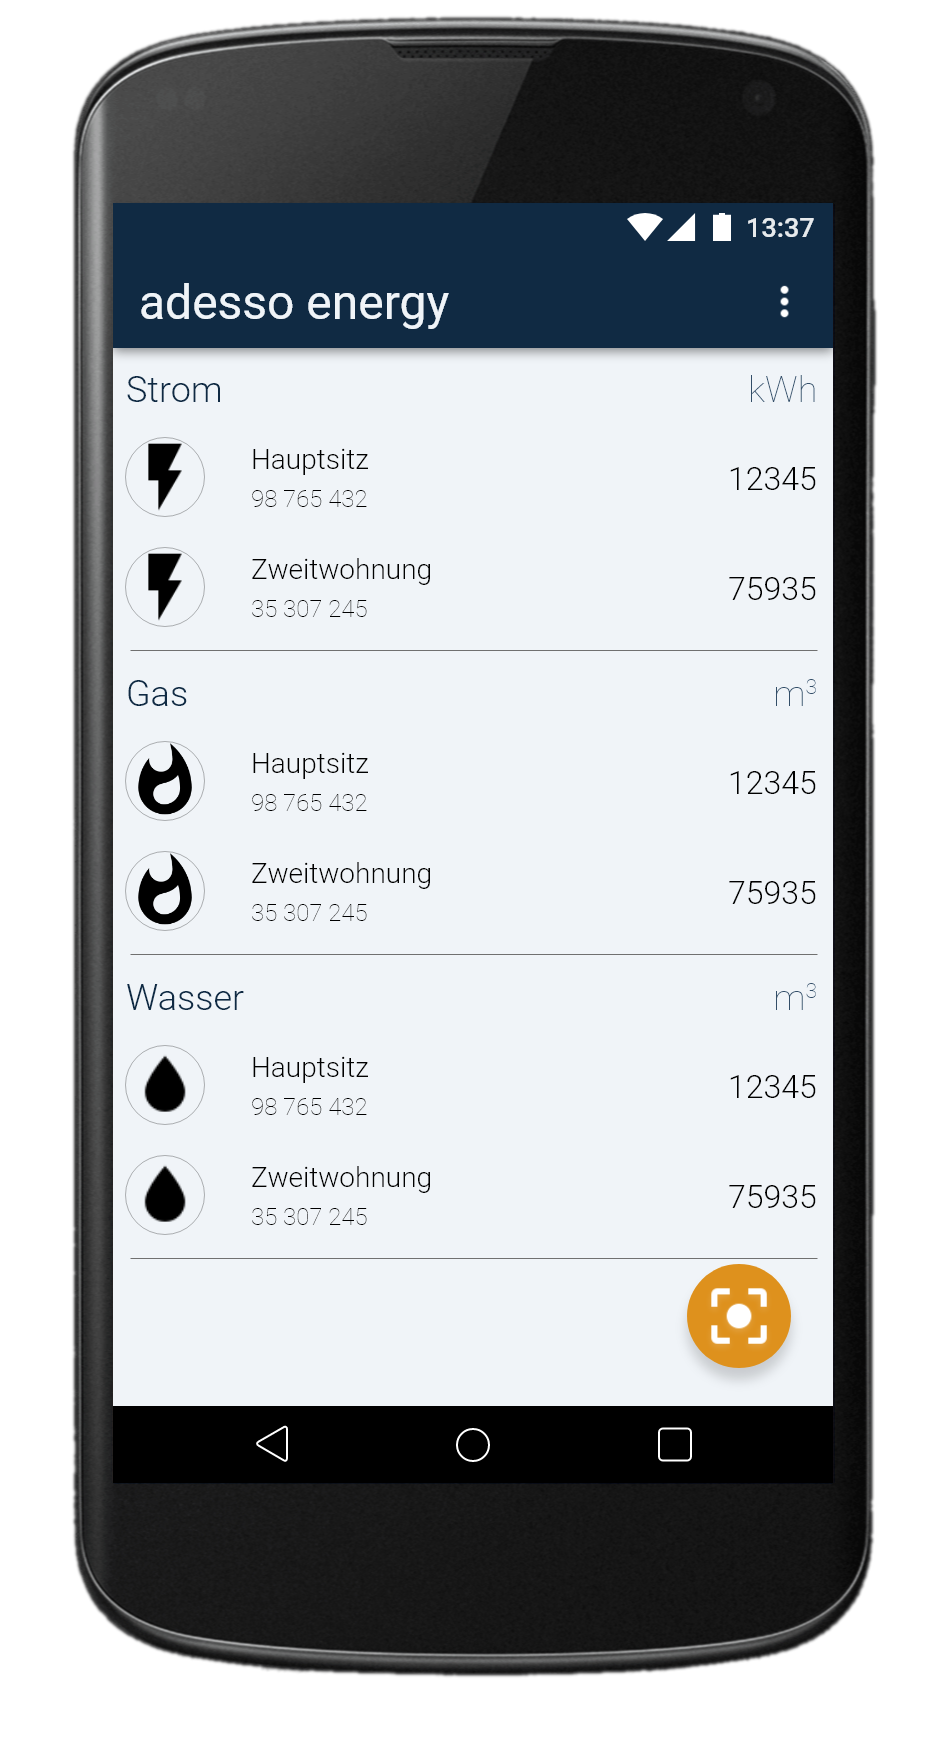
\includegraphics[scale = 0.22]{img/AndroidMockup/Main} & Dies ist der LoginBildschirm \\
\end{tabularx}
\end{figure}


\begin{figure}[h]
\begin{tabularx}{\textwidth}{X | X}
	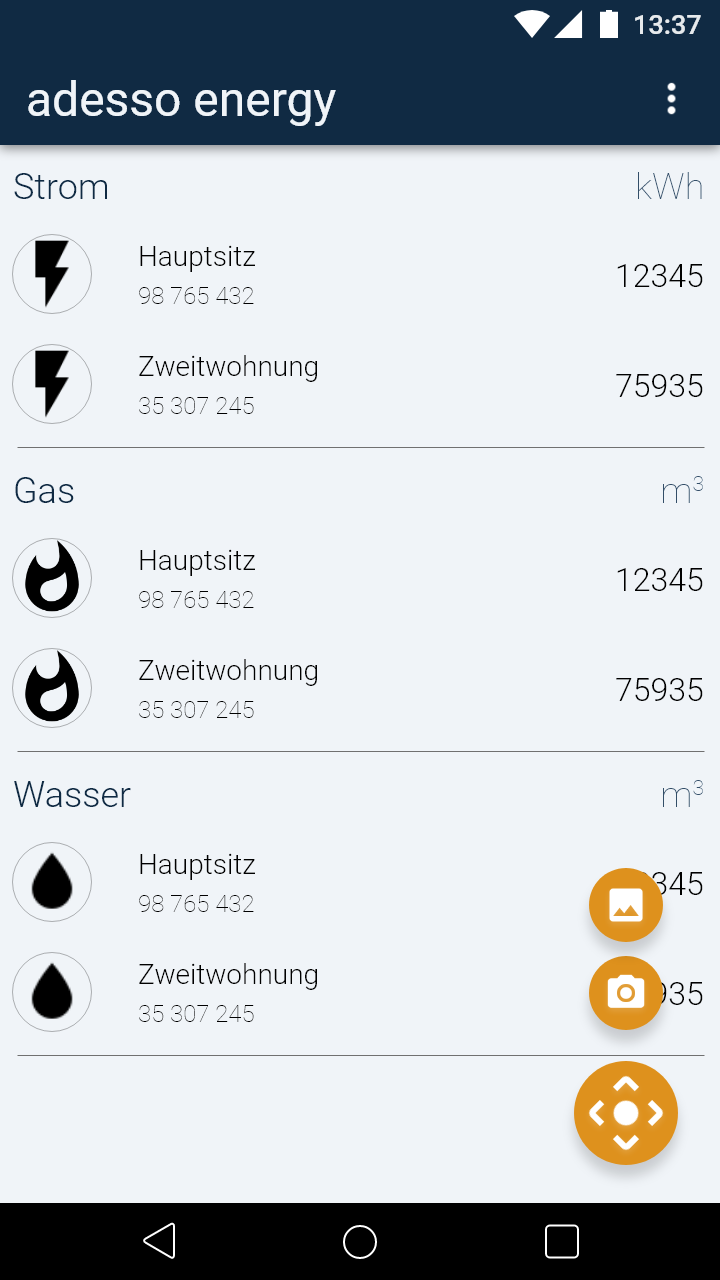
\includegraphics[scale = 0.22]{img/AndroidMockup/FABMenu} & Ganz viel Text. Ganz viel Text.Ganz viel Text.Ganz viel Text.Ganz viel Text.Ganz viel Text.Ganz viel Text.Ganz viel Text. \\ \hline \\
	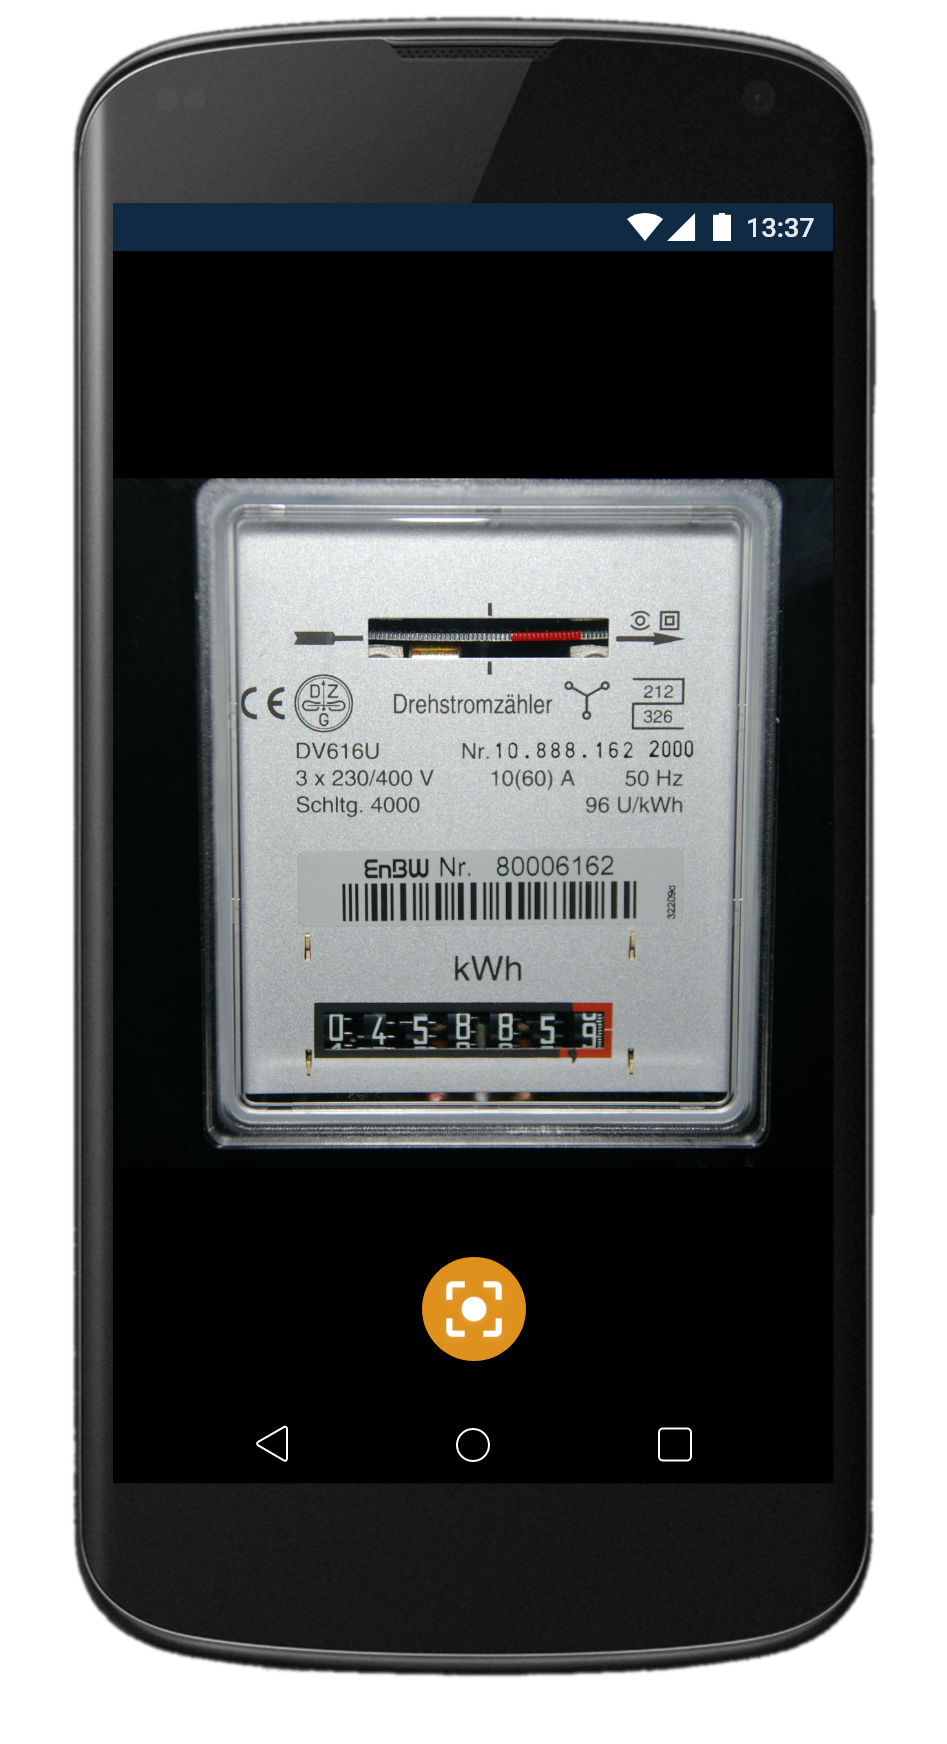
\includegraphics[scale = 0.22]{img/AndroidMockup/SystemCamera} & Dies ist der LoginBildschirm \\ 
\end{tabularx}
\end{figure}

\begin{figure}[h]
\begin{tabularx}{\textwidth}{X | X}
	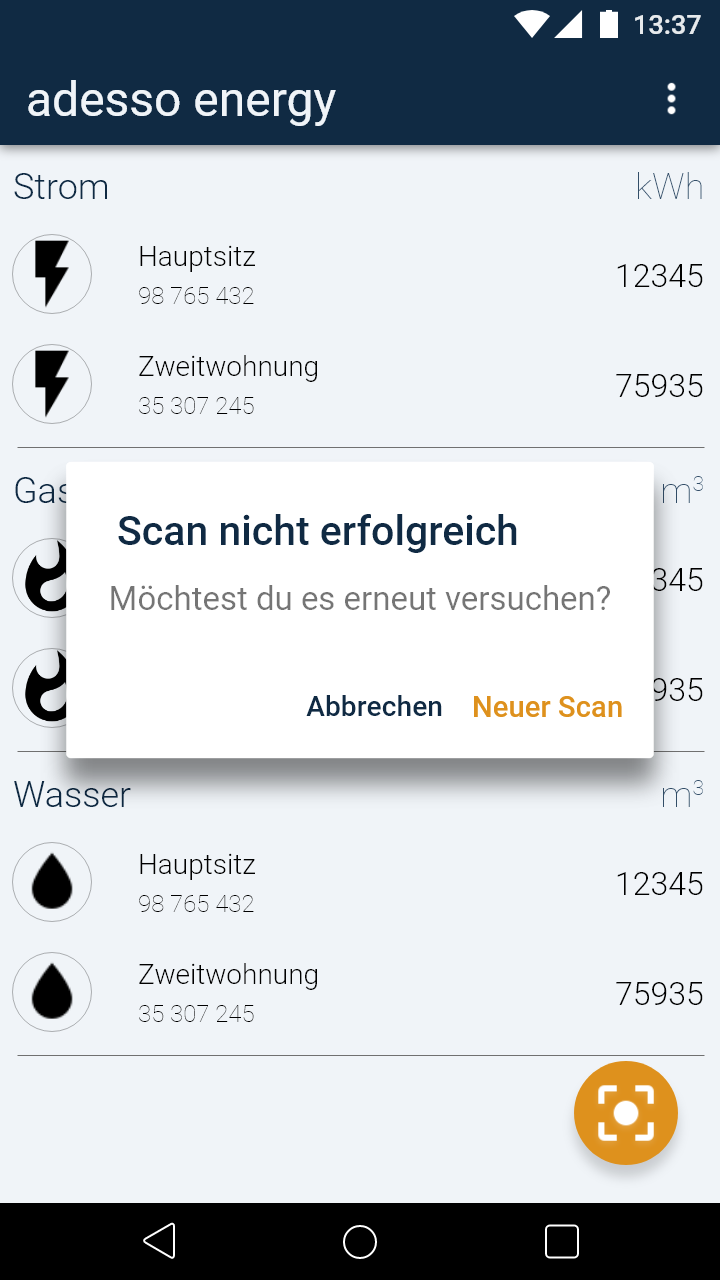
\includegraphics[scale = 0.22]{img/AndroidMockup/imageFailed} & Ganz viel Text. Ganz viel Text.Ganz viel Text.Ganz viel Text.Ganz viel Text.Ganz viel Text.Ganz viel Text.Ganz viel Text. \\ \hline \\
	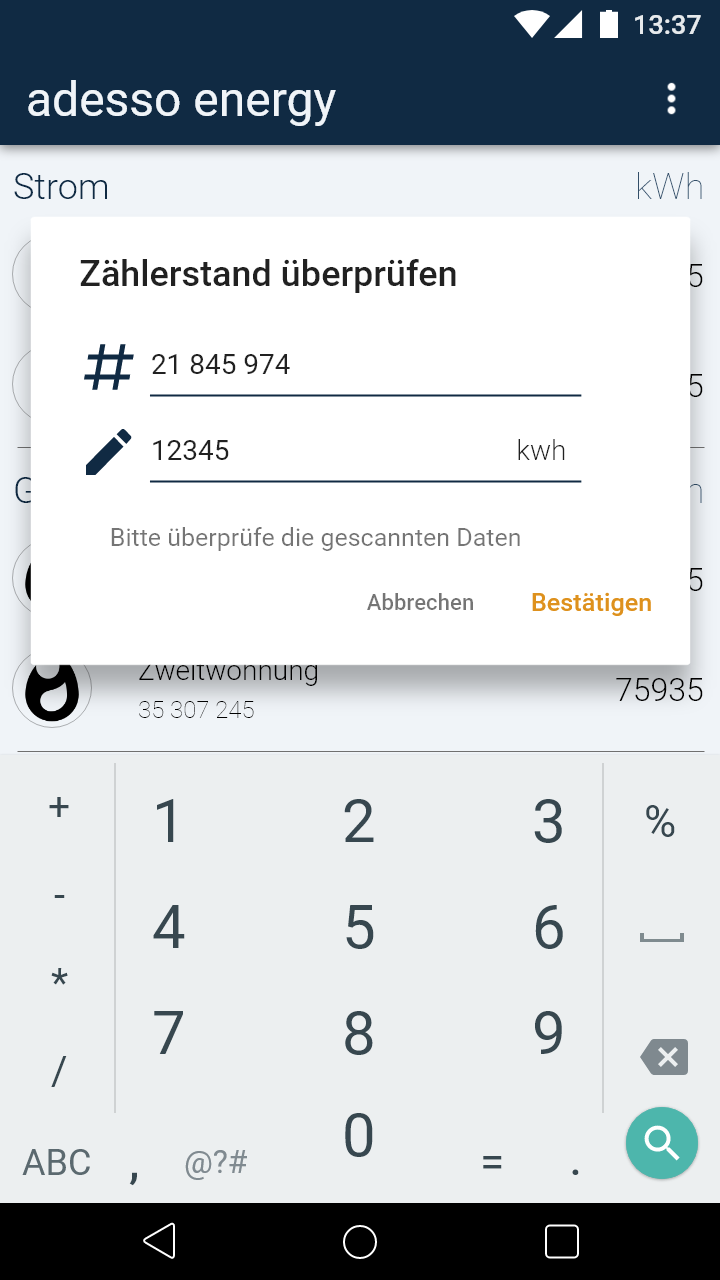
\includegraphics[scale = 0.22]{img/AndroidMockup/check} & Dies ist der LoginBildschirm \\ 
\end{tabularx}
\end{figure}

\begin{figure}[h]
\begin{tabularx}{\textwidth}{X | X}
	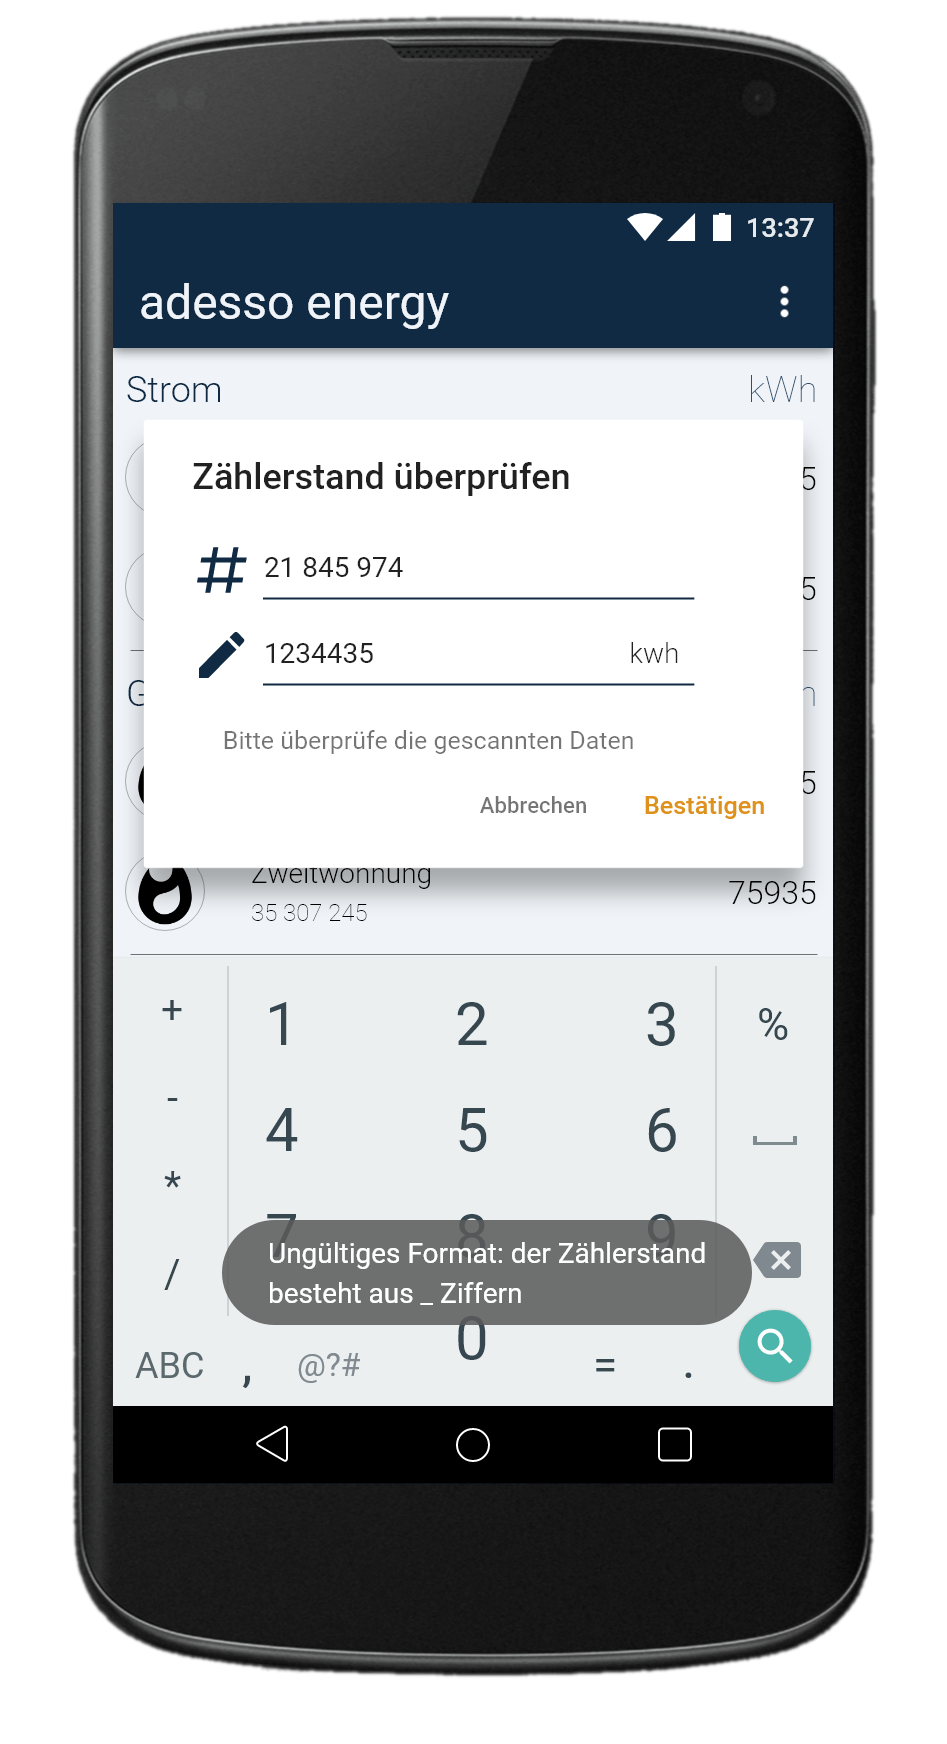
\includegraphics[scale = 0.22]{img/AndroidMockup/illegalFormatException} & Ganz viel Text. Ganz viel Text.Ganz viel Text.Ganz viel Text.Ganz viel Text.Ganz viel Text.Ganz viel Text.Ganz viel Text. \\ \hline \\
	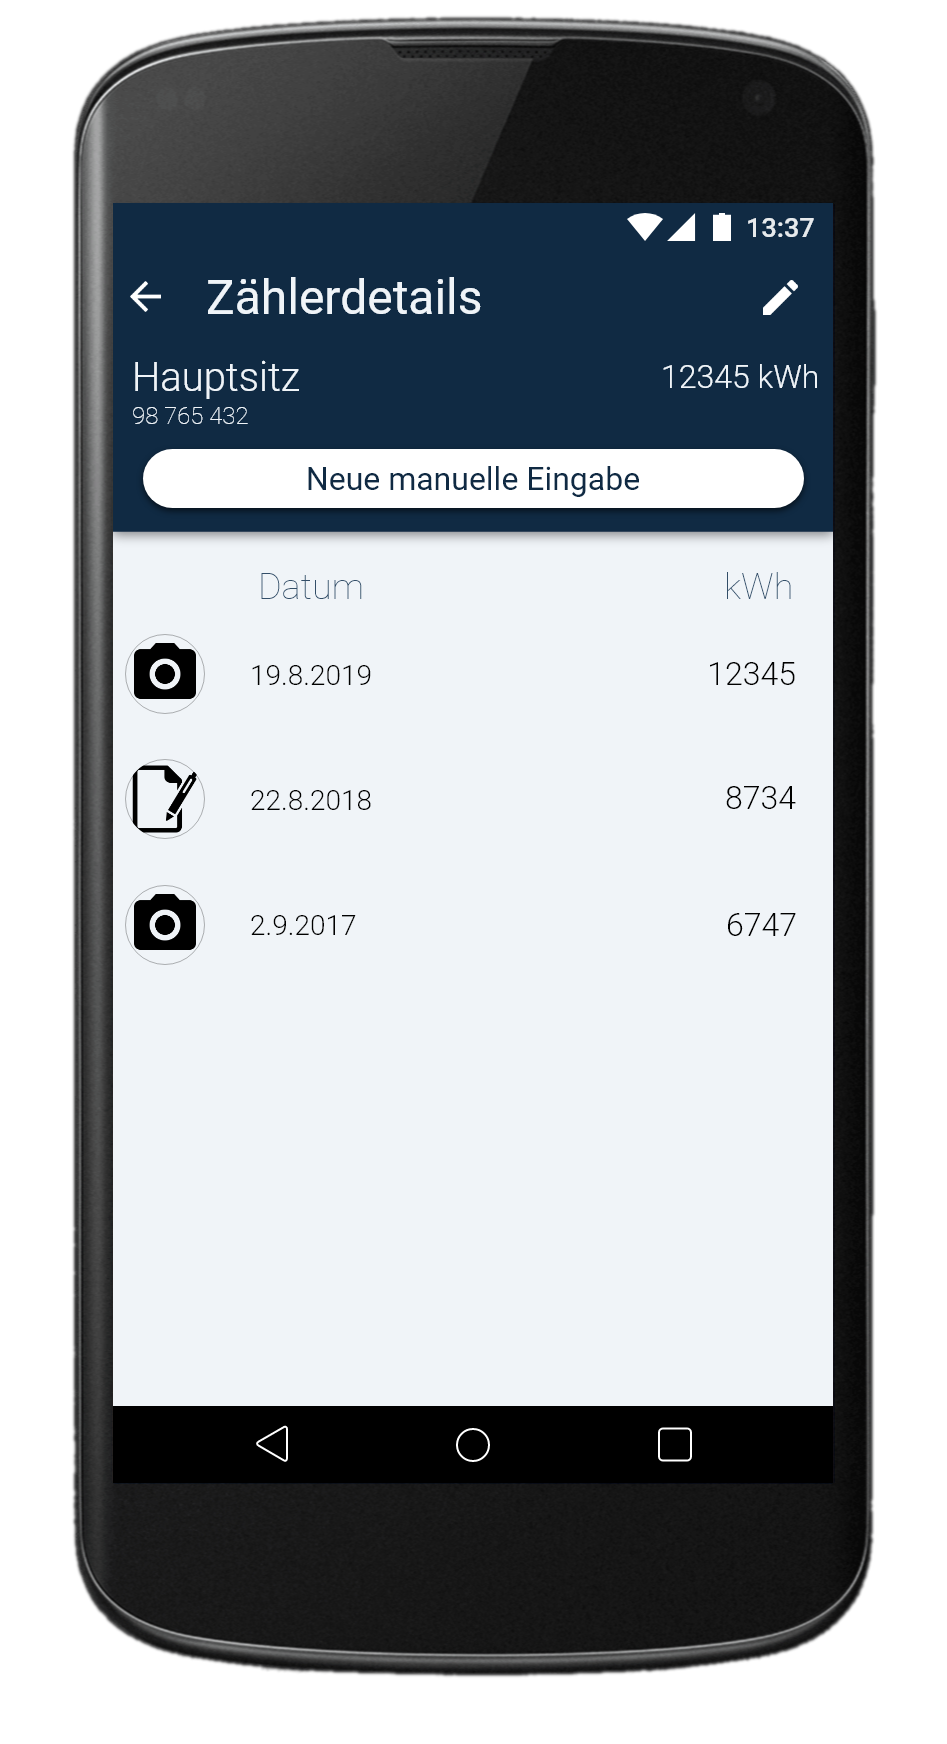
\includegraphics[scale = 0.22]{img/AndroidMockup/history} & Dies ist der LoginBildschirm \\
\end{tabularx}
\end{figure}

\begin{figure}[h]
\begin{tabularx}{\textwidth}{X | X}
	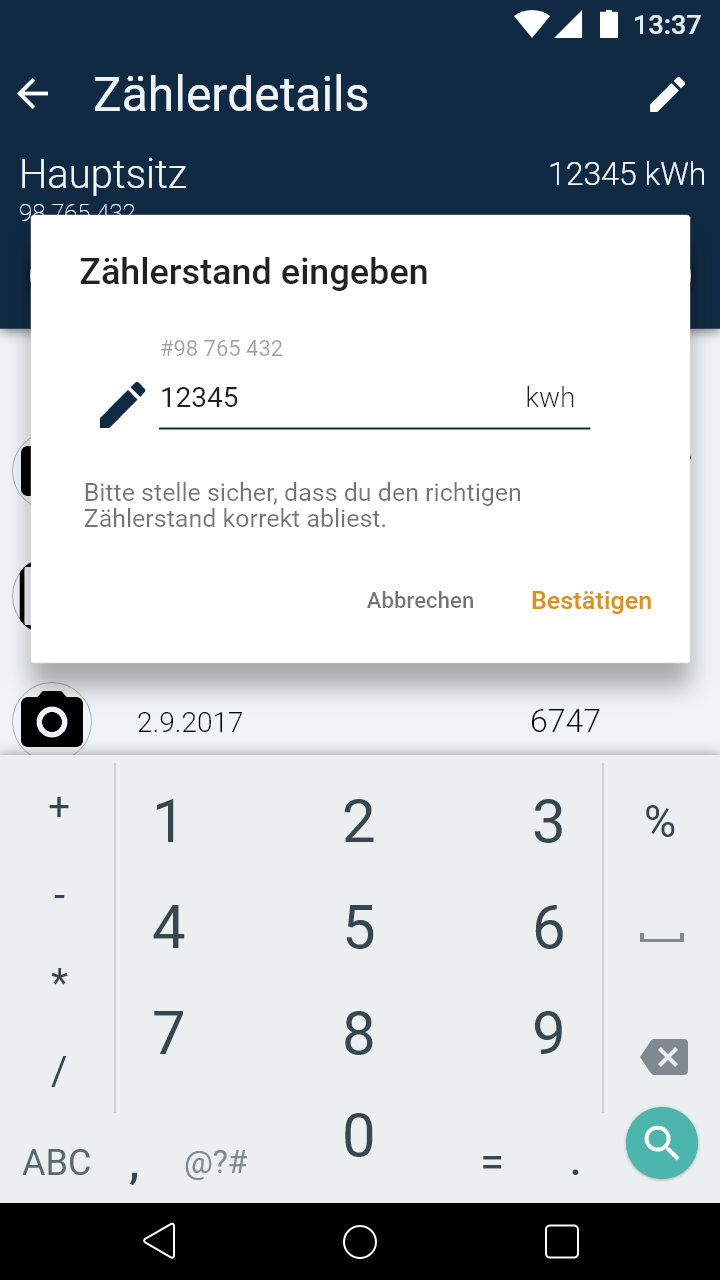
\includegraphics[scale = 0.22]{img/AndroidMockup/manuelEntry} & Ganz viel Text. Ganz viel Text.Ganz viel Text.Ganz viel Text.Ganz viel Text.Ganz viel Text.Ganz viel Text.Ganz viel Text. \\ \hline \\
	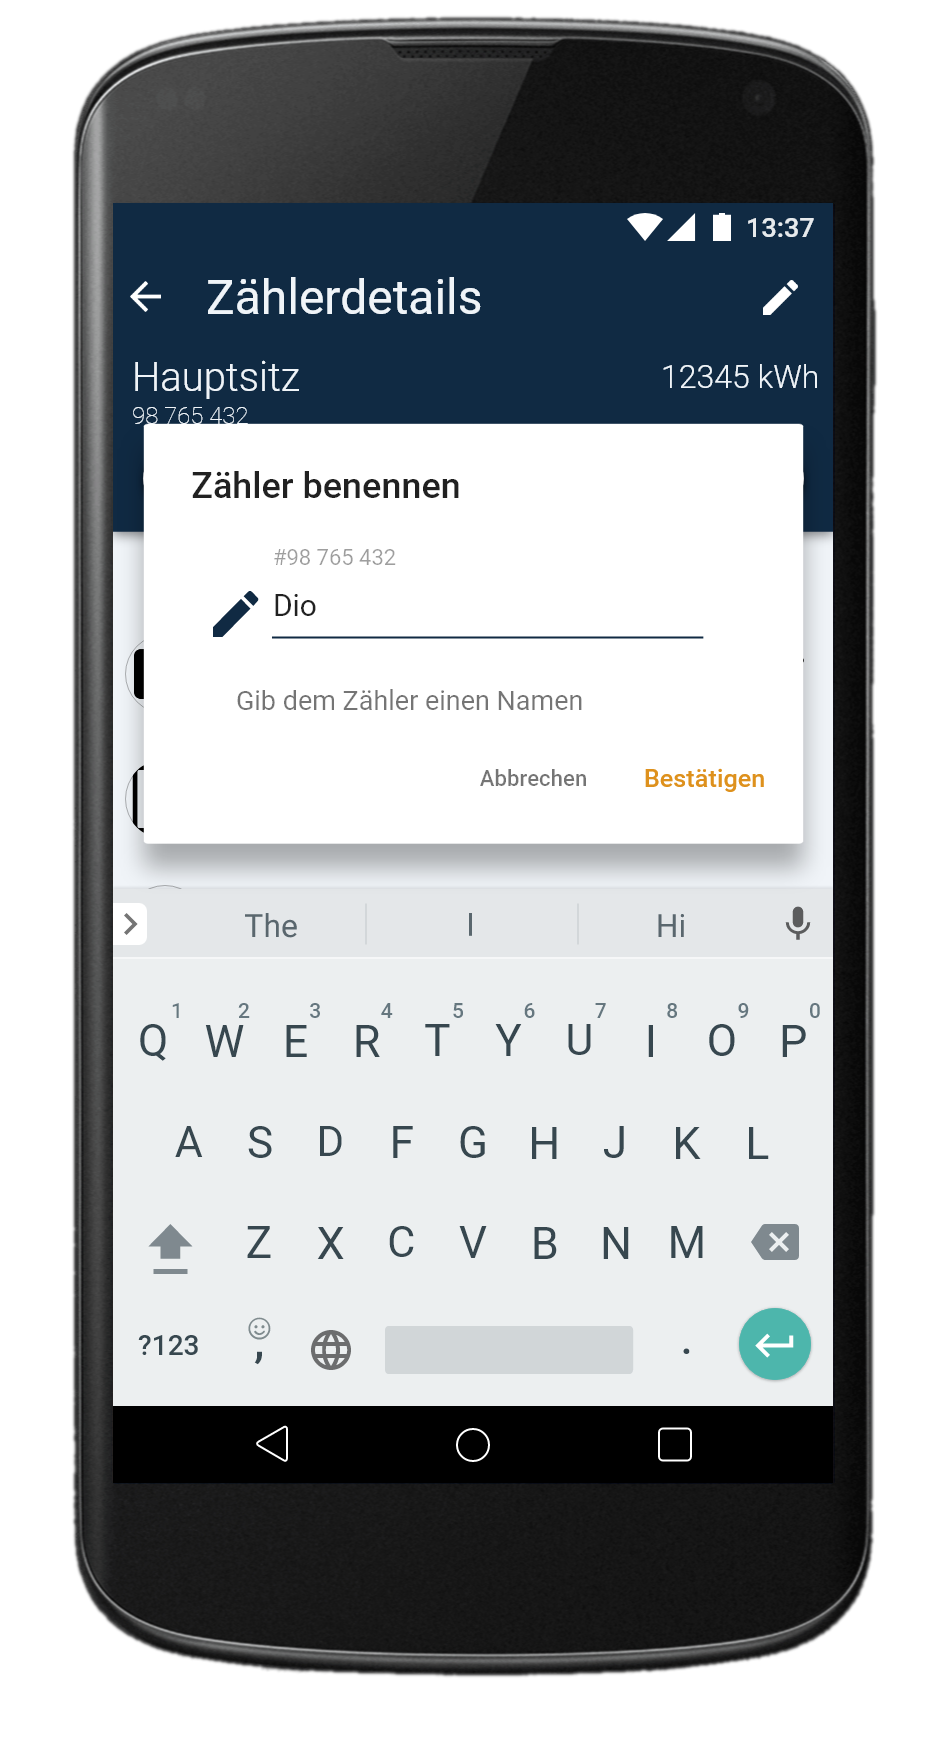
\includegraphics[scale = 0.22]{img/AndroidMockup/rename} & Dies ist der LoginBildschirm \\ 
\end{tabularx}
\end{figure}

\begin{figure}[h]
\begin{tabularx}{\textwidth}{X | X}
	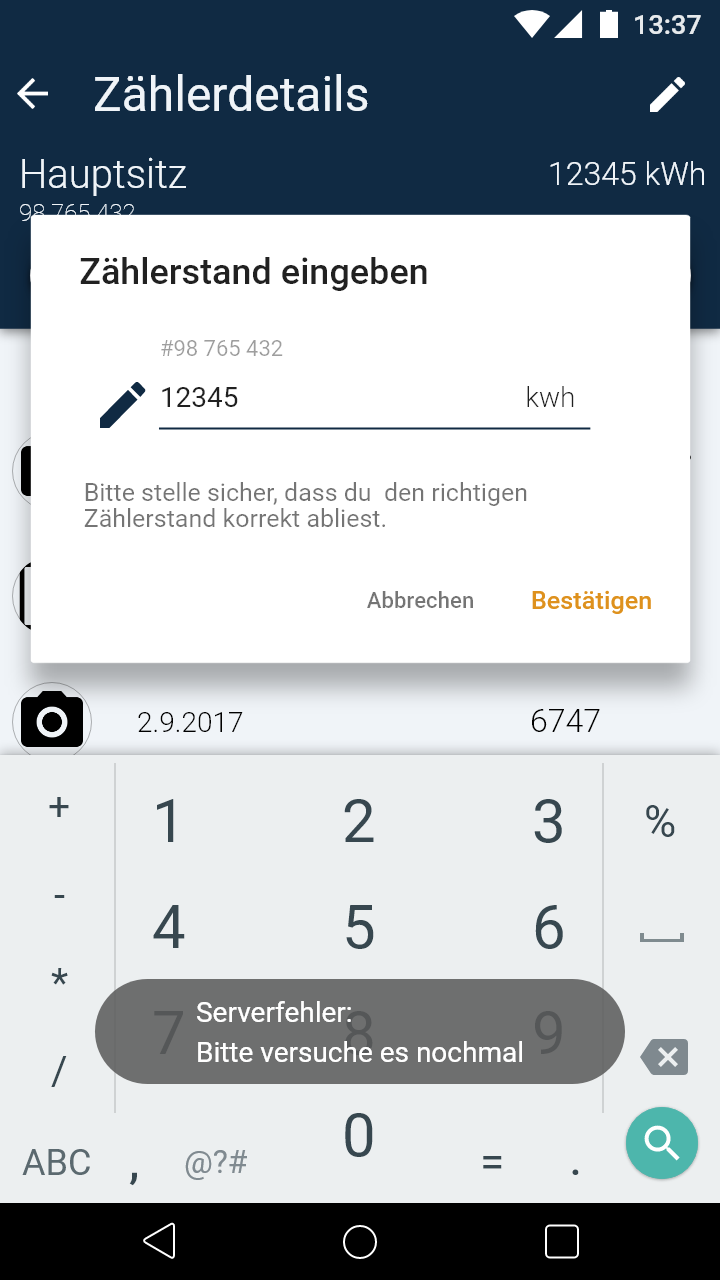
\includegraphics[scale = 0.22]{img/AndroidMockup/serverException} & Ganz viel Text. Ganz viel Text.Ganz viel Text.Ganz viel Text.Ganz viel Text.Ganz viel Text.Ganz viel Text.Ganz viel Text. \\ \hline \\
	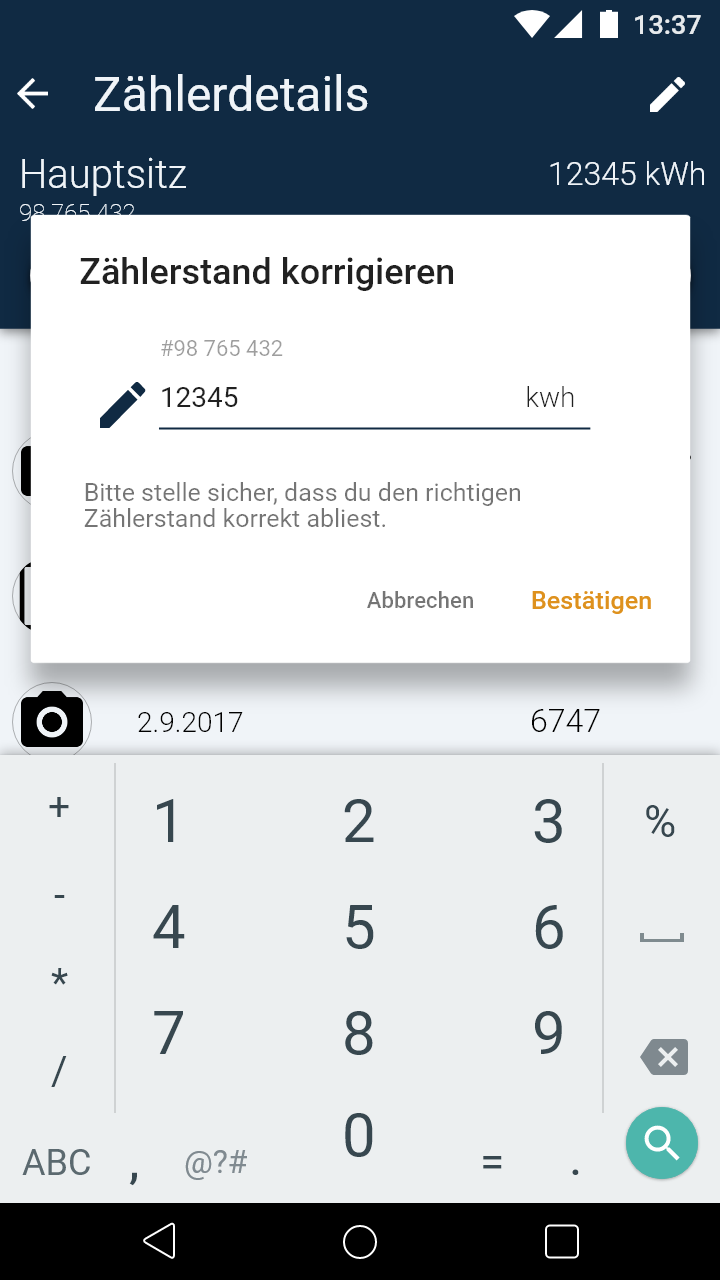
\includegraphics[scale = 0.22]{img/AndroidMockup/correct} & Dies ist der LoginBildschirm \\ 
\end{tabularx}
\end{figure}

\begin{figure}[h]
\begin{tabularx}{\textwidth}{X | X}
	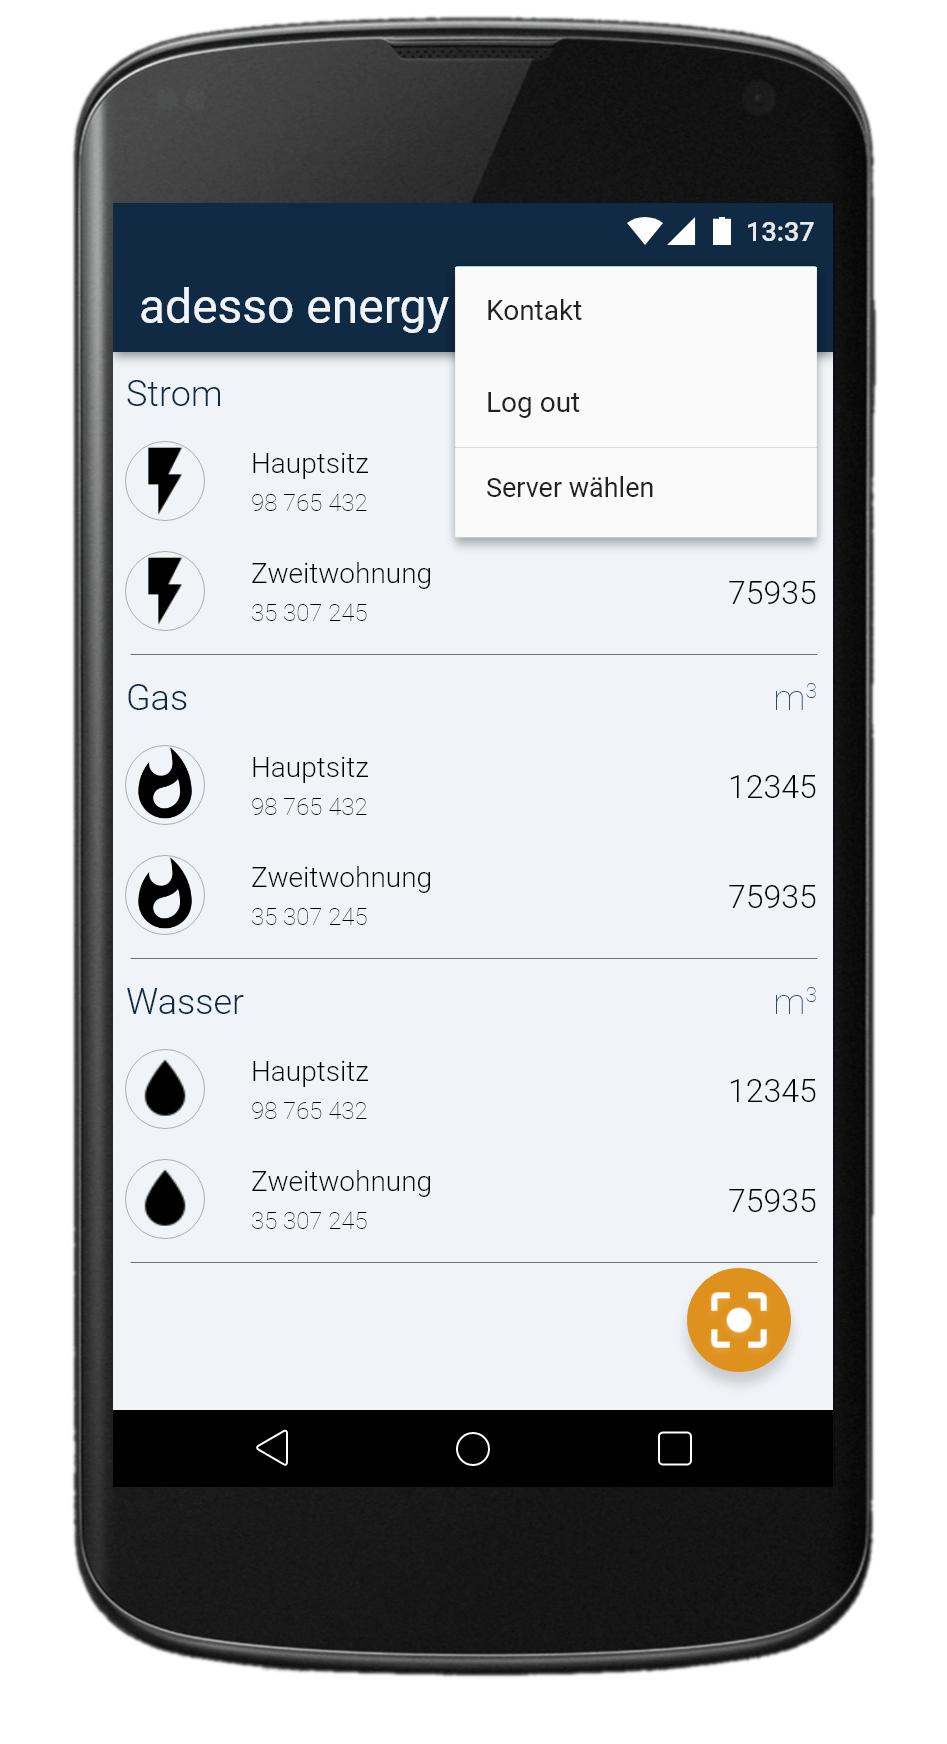
\includegraphics[scale = 0.22]{img/AndroidMockup/dropdown} & Ganz viel Text. Ganz viel Text.Ganz viel Text.Ganz viel Text.Ganz viel Text.Ganz viel Text.Ganz viel Text.Ganz viel Text. \\ \hline \\
	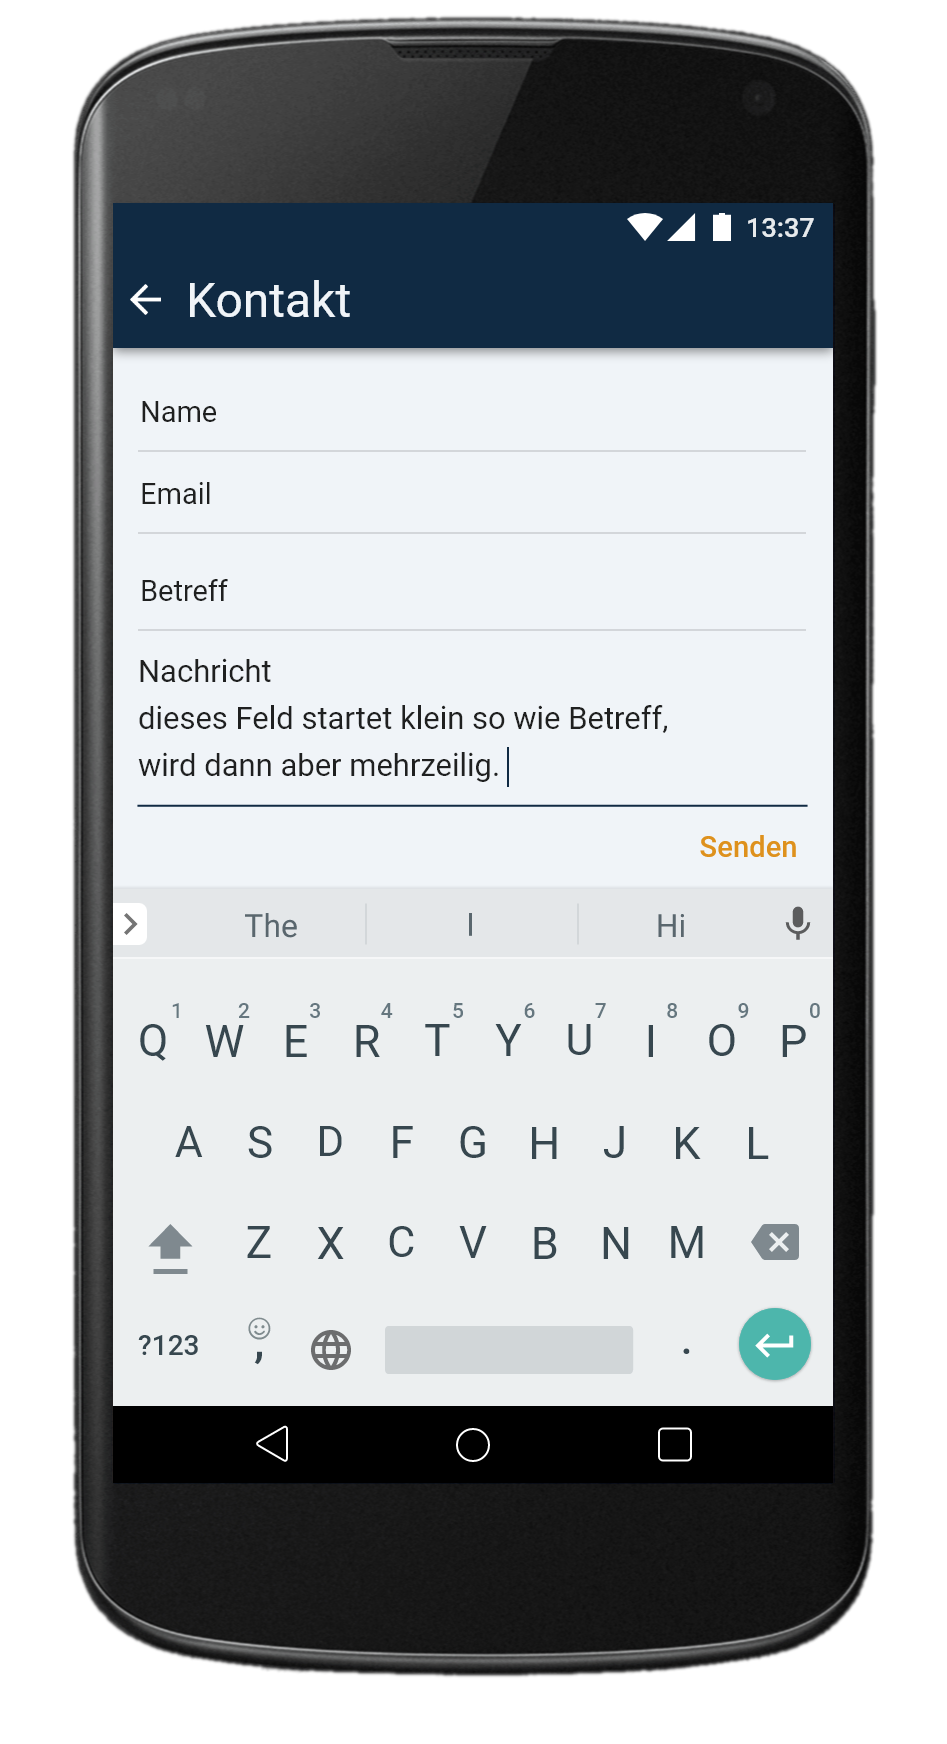
\includegraphics[scale = 0.22]{img/AndroidMockup/contact} & Dies ist der LoginBildschirm \\ 
\end{tabularx}
\end{figure}

\begin{figure}[h]
\begin{tabularx}{\textwidth}{X | X}
	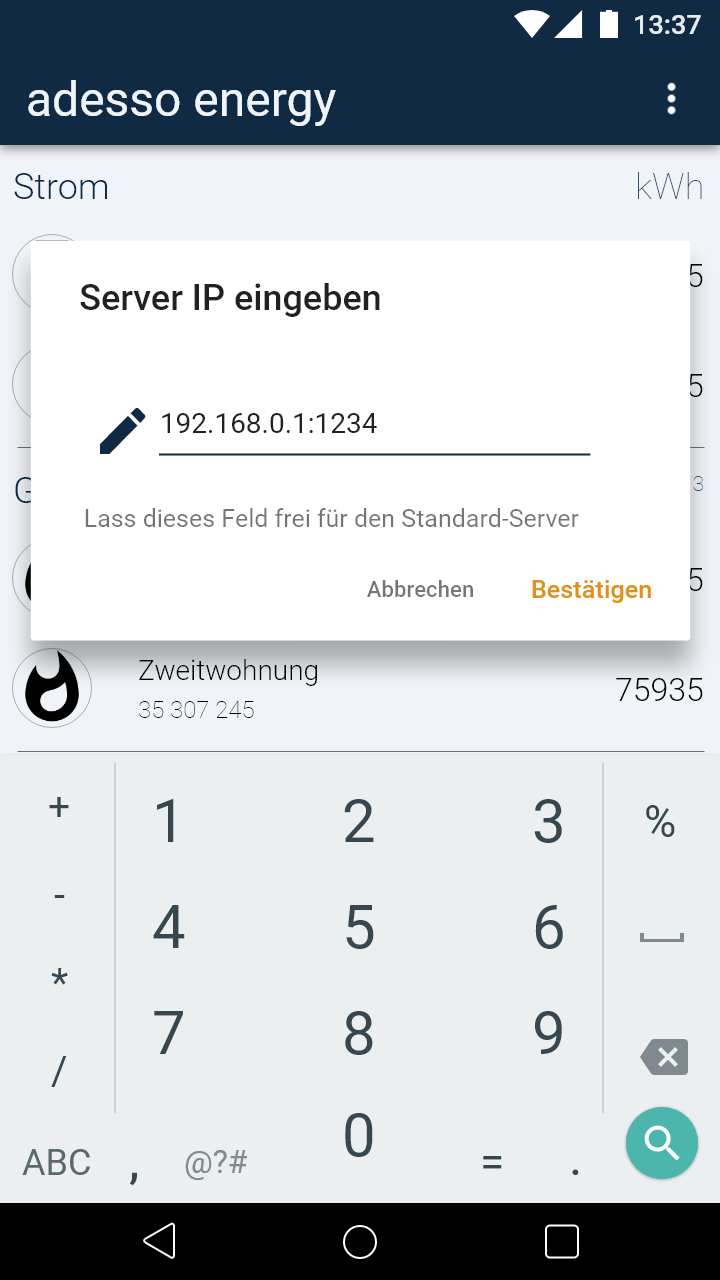
\includegraphics[scale = 0.22]{img/AndroidMockup/serverLocation} & Ganz viel Text. Ganz viel Text.Ganz viel Text.Ganz viel Text.Ganz viel Text.Ganz viel Text.Ganz viel Text.Ganz viel Text.
\end{tabularx}
\end{figure}



